\chapter{Examples and Workflows}

\section{Gyroid (Ia-3d)}

The gyroid is a bicontinuous minimal surface with Ia-3d symmetry. It is one of the most studied structures in block copolymer science.

\subsection{Generation Steps}

\begin{enumerate}
    \item Load space group operations from \texttt{examples/space\_groups\_3d/ia\_3d.txt}
    \item Load lattice parameters (cubic, $a = 10$)
    \item Build basis: find all valid stars up to $N_{\text{max}} = 5$
    \item Random initialization: assign random amplitudes with symmetry constraints
    \item Build field: compute inverse FFT on $64^3$ grid
    \item Normalize: apply tanh normalization
    \item Export: write to \texttt{gyroid.vts}
\end{enumerate}

\subsection{Expected Results}

\begin{itemize}
    \item 5 modes (families) with multiplicities: 8, 6, 24, 12, 48
    \item Total Fourier modes: 98
    \item Field range: $[0, 1]$ after normalization
    \item Square norm: $\approx 0.5$ for random initialization
\end{itemize}

\subsection{Symmetry Analysis}

The Ia-3d space group has 16 symmetry operations. The gyroid structure is characterized by:
\begin{itemize}
    \item No reflection planes (chiral structure)
    \item Three-fold screw axes along $\langle 111 \rangle$ directions
    \item Two-fold rotation axes along $\langle 110 \rangle$ directions
    \item Inversion center at the origin
\end{itemize}

The gyroid minimal surface is defined by:
\begin{equation}
    \cos(x+y)\cos(y+z) + \cos(y+z)\cos(x+z) + \cos(x+z)\cos(x+y) = 0
\end{equation}

\section{BCC-like (Pm-3m)}

The Pm-3m space group generates BCC-like density modulations.

\subsection{Generation Steps}

Same as gyroid, but with \texttt{pm3m.txt} space group file and cubic lattice.

\subsection{Expected Results}

\begin{itemize}
    \item Simple cubic symmetry with mirror planes in all three directions
    \item Field shows spherical density maxima at BCC lattice points
    \item Useful for studying sphere-forming block copolymers
\end{itemize}

\section{2D Examples}

\subsection{Square Lattice (P4)}

The P4 wallpaper group generates 4-fold symmetric patterns.

\begin{itemize}
    \item 4 symmetry operations (0\textdegree, 90\textdegree, 180\textdegree, 270\textdegree rotations)
    \item Supports 2D field generation
    \item Useful for studying 2D self-assembly patterns
\end{itemize}

\begin{verbatim}
# Run the 2D P4 example
source /sandbox/setup_build.sh
make
./examples/run_2d_p4.sh
\end{verbatim}

\subsection{Hexagonal Lattice (P6)}

The P6 wallpaper group generates 6-fold symmetric patterns.

\begin{itemize}
    \item 6 symmetry operations (0\textdegree, 60\textdegree, 120\textdegree, 180\textdegree, 240\textdegree, 300\textdegree)
    \item Supports 2D field generation
    \item Hexagonal packing patterns
\end{itemize}

\begin{verbatim}
# Run the 2D P6 example
source /sandbox/setup_build.sh
make
./examples/run_2d_p6.sh
\end{verbatim}

\subsection{Rectangular Lattice (Pmm2)}

The Pmm2 wallpaper group generates patterns with two perpendicular mirror lines.

\begin{itemize}
    \item 4 symmetry operations (identity, two mirrors, 2-fold rotation)
    \item Rectangular Bravais lattice
    \item Useful for studying anisotropic patterns
\end{itemize}

\section{Workflow Summary}

\begin{figure}[h]
\centering
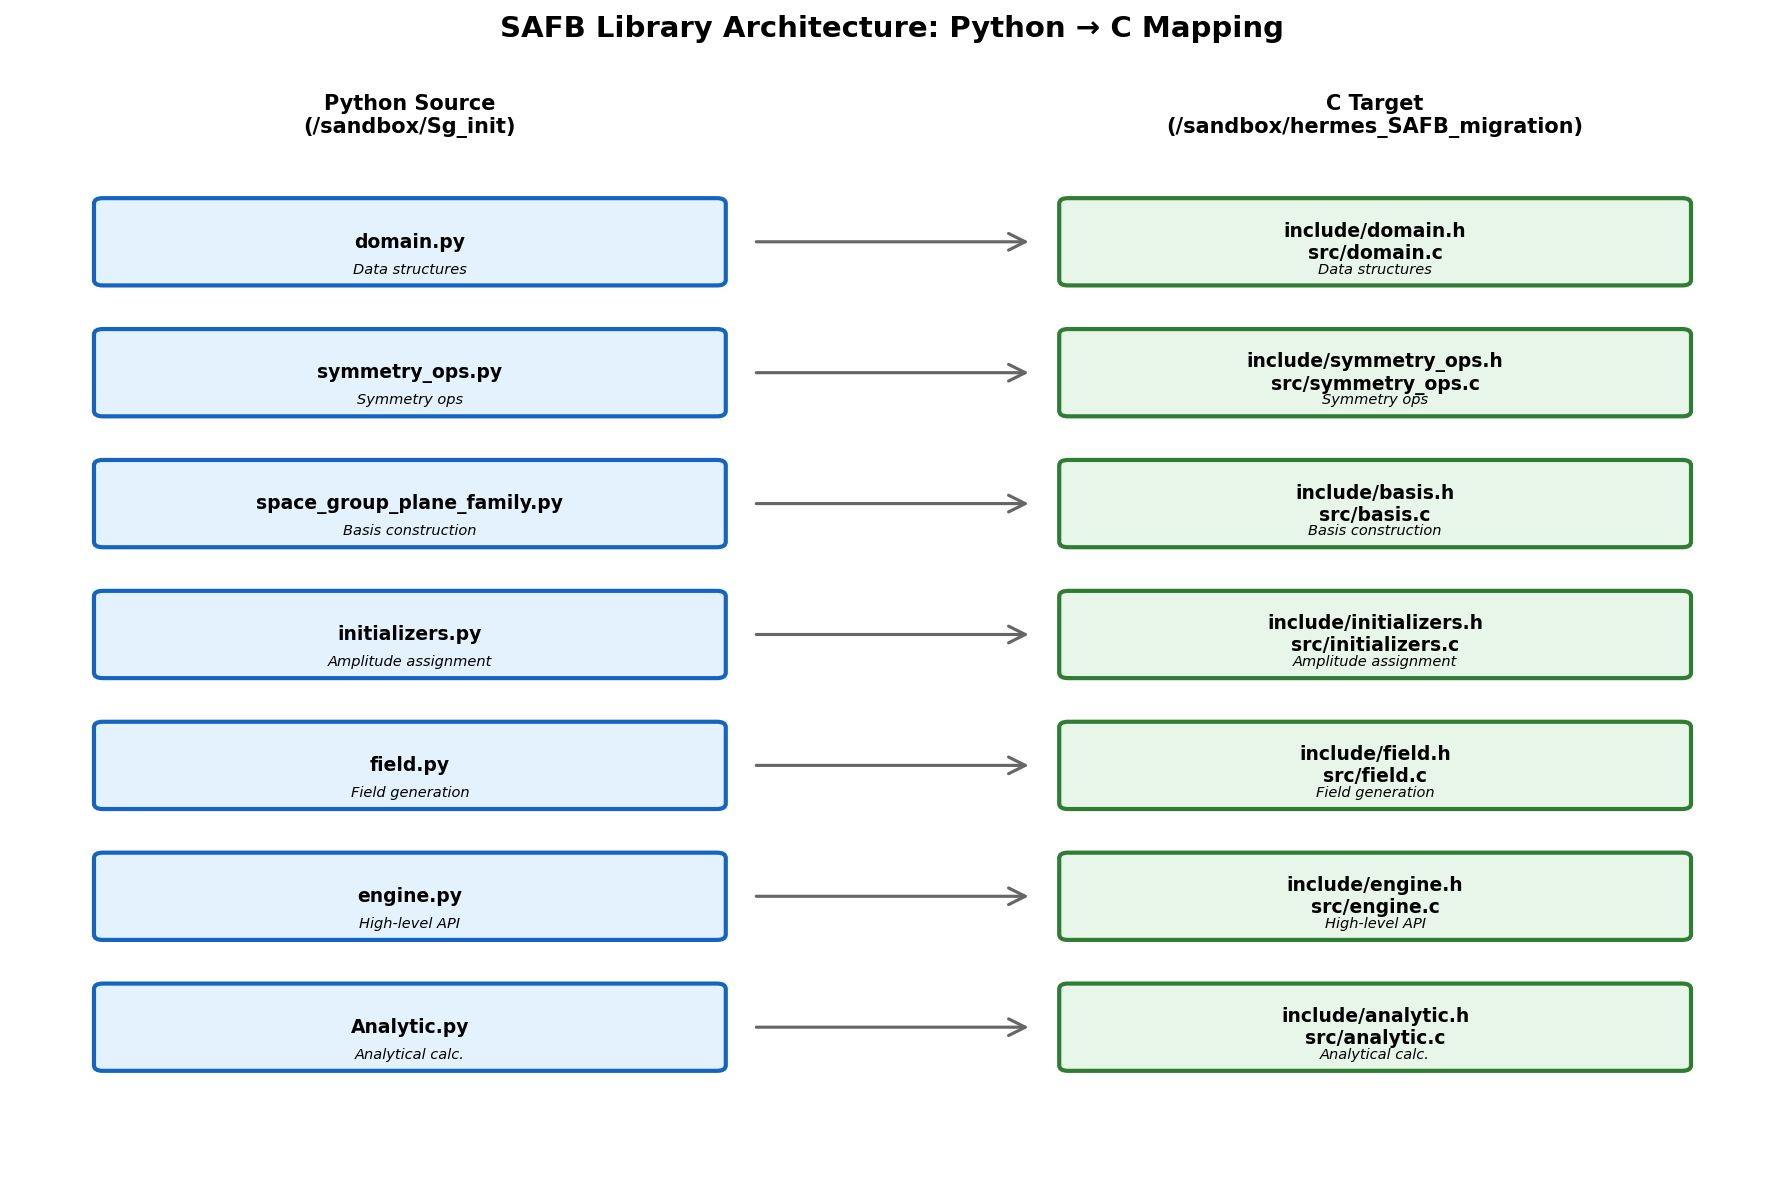
\includegraphics[width=0.8\textwidth]{architecture_diagram.png}
\caption{SAFB library architecture: Python-to-C module mapping.}
\end{figure}

\begin{figure}[h]
\centering
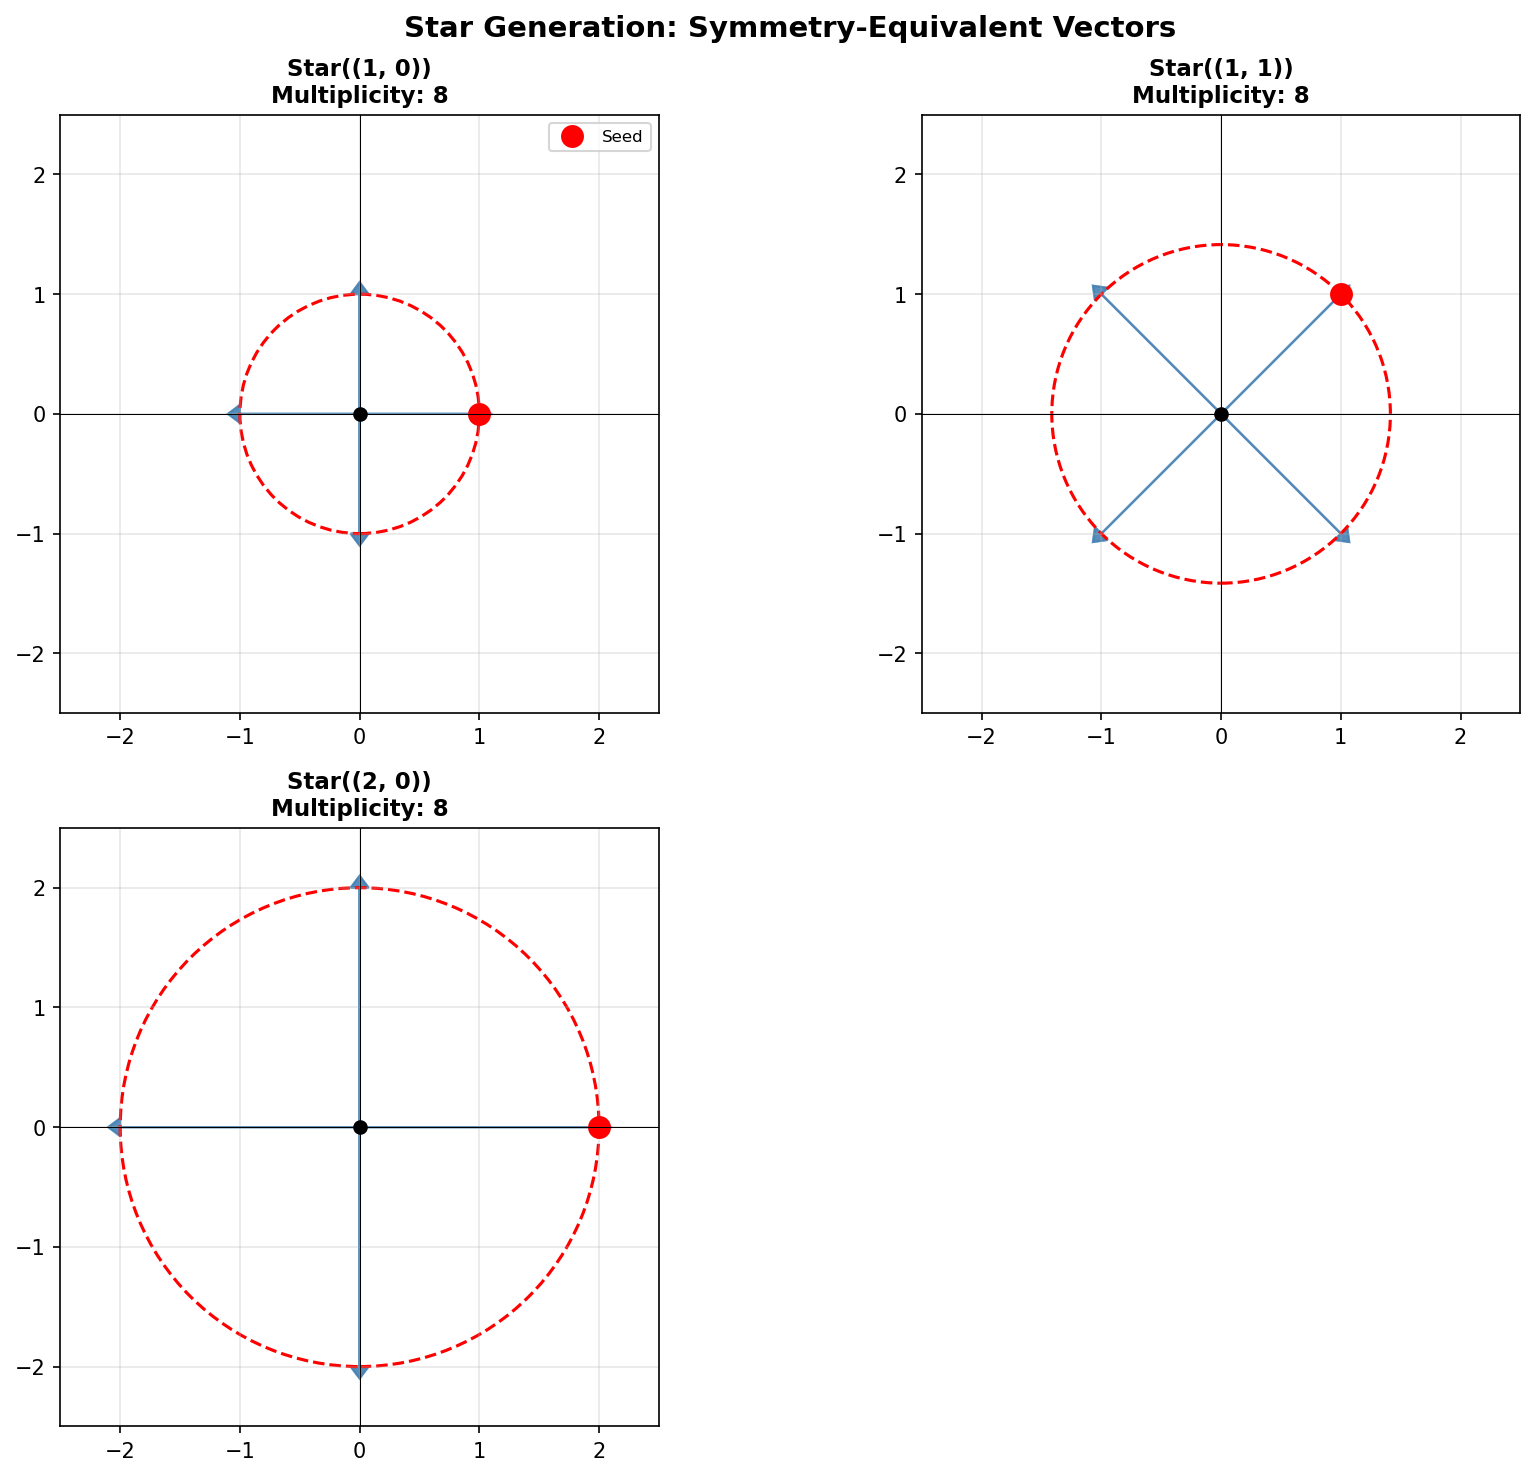
\includegraphics[width=0.8\textwidth]{star_generation.png}
\caption{Star generation: symmetry-equivalent vectors in reciprocal space.}
\end{figure}

The typical workflow is:

\begin{enumerate}
    \item \textbf{Setup}: Source the build environment and compile the library
    \item \textbf{Configure}: Set lattice parameters and grid resolution
    \item \textbf{Initialize}: Choose an initialization method (random, manual, or file-based)
    \item \textbf{Generate}: Compute the real-space field via inverse FFT
    \item \textbf{Visualize}: Export to VTK format and view in ParaView
\end{enumerate}

\section{Parameter Tuning}

\subsection{Grid Resolution}

Higher grid resolution gives more accurate fields but increases computation time:

\begin{table}[h]
\centering
\begin{tabular}{lll}
\hline\hline
\textbf{Resolution} & \textbf{3D Time (est.)} & \textbf{Use Case} \\
\hline
$16^3$ & $\sim 0.1$s & Testing, development \\
$32^3$ & $\sim 0.5$s & Quick prototyping \\
$64^3$ & $\sim 2$s & Production runs \\
$128^3$ & $\sim 15$s & High-precision studies \\
\hline\hline
\end{tabular}
\caption{Estimated computation times for different grid resolutions.}
\end{table}

\subsection{Number of Stars}

More stars (higher $N_{\text{max}}$) give more accurate representations but increase the number of free parameters:

\begin{itemize}
    \item $N_{\text{max}} = 3$: Few modes, smooth fields, fast convergence
    \item $N_{\text{max}} = 5$: Moderate resolution, typical for SCFT
    \item $N_{\text{max}} = 8$: High resolution, for detailed studies
\end{itemize}

\subsection{Scaling Parameter}

The tanh normalization parameter $\sigma$ controls the sharpness of the field:

\begin{itemize}
    \item $\sigma = 0.5$: Smooth transitions, low contrast
    \item $\sigma = 1.0$: Moderate contrast (default)
    \item $\sigma = 2.0$: Sharp interfaces, high contrast
\end{itemize}
